\appendix
\chapter{Applied in CPlan}
\section{Guideline Source Code}
This section provides a guideline through the important parts of the C\# source code, which was developed during this thesis. It's meant as an entry point which can be used to navigate more easily through the code, which implements the discussed concepts.

The main solution should be opened with Visual Studio from: 
\path{GIT_REPO\cpg_all\BasicSystems\SynthesisWPF\SynthesisWPF\SynthesisWPF.sln}

\gls{GUI} components were inserted into the sub-project Synthesis\_WPF\_MVVM. These dialogs were created in the sub folder \textit{Dialogs}:

\begin{itemize}
    \item K-Means Clustering Options (section \ref{sec:k-means_clustering_options})
    \item Hierarchical Clustering Options (section \ref{sec:hierarchical_clustering_options})
    \item Cluster Measurement Options (section \ref{sec:cluster_measurement_options})
    \item Measured Clusters (section \ref{sec:measurements_full_table})
\end{itemize}

Algorithms were inserted into the sub-project \textit{Optimization}. These classes / interfaces have been created for this thesis:
\begin{itemize}
    \item Tree representation of a graph (model) \newline
    \path{.\Chromosomes\InstructionTreePisaAbs.cs}
    \item Tree creating class from graph \newline
    \path{.\Chromosomes\TreeGenerator.cs}
    \item Class to recreate a graph from a tree \newline
    \path{.\Generators\StreetPatternAbsoluteAngle.cs}
    \item Helper class to extract blocks from a graph \newline
    \path{.\ClusterAnalysis\BlockAnalysis.cs}
    \item This class allows to get and export cluster analysis data \newline 
    \path{.\ClusterAnalysis\ClusterAnalysisExporter.cs}
    \item  Class to create feature based clusters \newline 
    \path{.\ClusterAnalysis\FeatureClustering.cs}
    \item Hierarchical clustering class \newline 
    \path{.\ClusterAnalysis\HierarchicalCluster.cs}
    \item Generic interface for cluster algorithms\newline
    \path{.\ClusterAnalysis\IClusterAnglorithm.cs}
    \item Generic hierarchical cluster output interface \newline 
    \path{.\ClusterAnalysis\IHierarchicalClusterOutput.cs}
    \item K-Means clustering class \newline
    \path{.\ClusterAnalysis\KMeansCluster.cs}
    \item Single Linkage clustering class \newline
    \path{.\ClusterAnalysis\SingleLinkageCluster.cs}
\end{itemize}

\pagebreak
\section{K-Means Clustering Options} \label{sec:k-means_clustering_options}
To apply centroid based clustering to a street network a specialized \gls{GUI} dialog was created where all parameters can be set. As you can see in figure \ref{fig:applied_k-means_GUI}.
\begin{itemize}
    \item If 'Show Visualisation' is activated the clustering process will be visualised.
    \item The counter 'Number of Tries' represents the count how often the clustering algorithm will be executed to extract the best result.
    \item 'Iterations per Try' describe how many iterations are maximal made per try.
    \item If 'Shortest Path' is selected, a shortest path algorithm will be applied after the centroid were set.
\end{itemize}
\begin{figure}[ht]
    \centering
    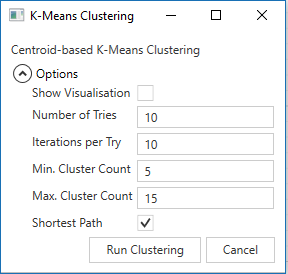
\includegraphics[width=0.47\linewidth]{k-means_clustering_applied.png}
    \caption{This \gls{GUI} dialog represents the parameters which could be applied to the K-Mean clustering algorithm.}
    \label{fig:applied_k-means_GUI}
\end{figure}

\pagebreak
\section{Hierarchical Clustering Options} \label{sec:hierarchical_clustering_options}
A specialised \gls{GUI} was created to set parameters for the hierarchical clustering analysis. The reduction formula can be selected at the top (figure \ref{fig:applied_HC_clustering_GUI}).

\begin{itemize}
    \item If the option 'Show Slider Dialog' is selected the cluster count can be changed in an additional dialog \ref{fig:applied_HC_clustering_slider_GUI}.
    \item The field 'Number of Clusters' represents the number of clusters which will be generated.
    \item If 'Modify Output' is selected, always the biggest cluster will be split instead as the hierarchy was created. The results are more equal cluster sizes.
\end{itemize}

\begin{figure}[ht]
    \centering
    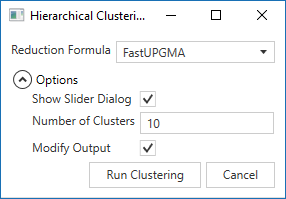
\includegraphics[width=0.47\linewidth]{HC_clustering_applied.png}
    \caption{This \gls{GUI} dialog represents the parameters which could be applied to the hierarchical clustering algorithm.}
    \label{fig:applied_HC_clustering_GUI}
\end{figure}

\begin{figure}[ht]
    \centering
    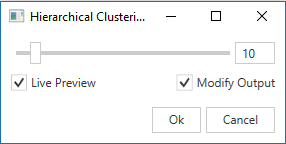
\includegraphics[width=0.47\linewidth]{HC_clustering_applied_slider.png}
    \caption{This \gls{GUI} dialog represents the optional 'Slide Dialog' which allows direct changes of the cluster count.}
    \label{fig:applied_HC_clustering_slider_GUI}
\end{figure}

\pagebreak
\section{Speed Measurements} \label{sec:speed_measurement_tables}

In section \ref{sec:measurements-speed} speed measurements were described evaluated. Tables \ref{tab:speed_measurements_kmeans} and \ref{tab:speed_measurements_hierarchical_clustering} list the original measurement data for the sake of completeness.

The following environment was used for these measurements:

\begin{itemize}
    \item \textbf{.Net Framework Version:} 4.6
    \item \textbf{Architecture:} 64-bit (x86-64)
    \item \textbf{Operating System:} Windows 10
    \item \textbf{Hardware Model:} Acer Aspire V3 772G
    \item \textbf{Processor:} Intel Core i7-4702MQ (Quad Core)
    \item \textbf{RAM:} 32 GB
\end{itemize}

\begin{table}[!hb]
    \centering
    \begin{tabular}{ | l | l | l | l | } \hline
        \textbf{Original} & \textbf{Parallel} & \textbf{Original \& Shortest Path} & \textbf{Parallel \& Shortest Path}  \\
        \hline

        29628 ms & 16104 ms & 33106 ms & 16838 ms \\
        28633 ms & 16268 ms & 31312 ms & 17135 ms \\
        28894 ms & 15959 ms & 31382 ms & 18046 ms \\
        29374 ms & 16149 ms & 32998 ms & 17590 ms \\
        29027 ms & 17704 ms & 32108 ms & 17991 ms \\
        28969 ms & 15937 ms & 32251 ms & 17923 ms \\
        28954 ms & 18308 ms & 32158 ms & 17291 ms \\
        29060 ms & 16462 ms & 31480 ms & 17132 ms \\
        30612 ms & 16756 ms & 33418 ms & 18817 ms \\
        28604 ms & 18461 ms & 31413 ms & 18280 ms \\
        \hline
    \end{tabular}
    \caption{K-Means Speed Measurements}
    \label{tab:speed_measurements_kmeans}
\end{table}

\begin{table}[!ht]
    \centering
    \begin{tabular}{ | l | l | l | l | } \hline
        \textbf{Variation} & \textbf{Original} & \textbf{Parallel} & \textbf{Original \& Shortest Path} \\
        \hline

        \multirow{10}{*}{\begin{minipage}{3cm}UPGMA (without distance caching)\end{minipage}}
        & 98618 ms & 63001 ms & 61006 ms \\
        & 100678 ms & 62909 ms & 60212 ms \\
        & 101714 ms & 63299 ms & 60778 ms \\
        & 98792 ms & 61560 ms & 62275 ms \\
        & 98842 ms & 61374 ms & 61336 ms \\
        & 98099 ms & 61835 ms & 61557 ms \\
        & 97791 ms & 61881 ms & 61784 ms \\
        & 97526 ms & 61623 ms & 61812 ms \\
        & 97946 ms & 61226 ms & 61629 ms \\
        & 97756 ms & 61813 ms & 62769 ms \\
        \hline

        \multirow{10}{*}{\begin{minipage}{3cm}UPGMA (fast / cached distances)\end{minipage}}
        & 15122 ms & 2172 ms & 865 ms \\
        & 15240 ms & 2124 ms & 852 ms \\
        & 15005 ms & 2135 ms & 864 ms \\
        & 14920 ms & 2126 ms & 870 ms \\
        & 15006 ms & 2132 ms & 853 ms \\
        & 15033 ms & 2107 ms & 863 ms \\
        & 15053 ms & 2101 ms & 844 ms \\
        & 15099 ms & 2117 ms & 860 ms \\
        & 15188 ms & 2089 ms & 859 ms \\
        & 15178 ms & 2095 ms & 857 ms \\
        \hline

        \multirow{10}{*}{\begin{minipage}{3cm}WPGMA (fast / cached distances)\end{minipage}}
        & 15012 ms & 2091 ms & 834 ms \\
        & 15036 ms & 2086 ms & 847 ms \\
        & 15179 ms & 2117 ms & 844 ms \\
        & 15152 ms & 2123 ms & 862 ms \\
        & 15135 ms & 2075 ms & 843 ms \\
        & 15239 ms & 2122 ms & 836 ms \\
        & 15074 ms & 2168 ms & 845 ms \\
        & 15065 ms & 2108 ms & 835 ms \\
        & 15099 ms & 2062 ms & 846 ms \\
        & 15051 ms & 2107 ms & 869 ms \\
        \hline
    \end{tabular}
    \caption{Hierarchical Clustering Speed Measurements}
    \label{tab:speed_measurements_hierarchical_clustering}
\end{table}

\pagebreak
\section{Cluster Measurement Options} \label{sec:cluster_measurement_options}
To compare clusters, the process was visualised for this thesis. A dialog allows to select two clusters and compare the measured results (figure \ref{fig:applied_clustering_analysis_GUI}). The selected clusters are marked by colours in the main view \ref{fig:applied_clustering_analysis_visualized_GUI}.

\begin{figure}[ht]
    \centering
    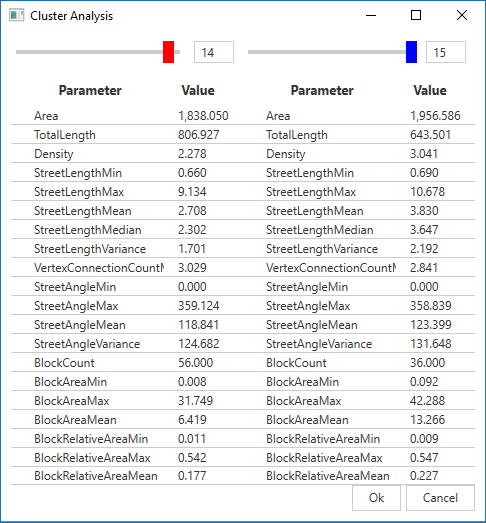
\includegraphics[width=0.8\linewidth]{cluster_applied_compare.png}
    \caption{This \gls{GUI} dialog allows to select two clusters and to compare the measured values.}
    \label{fig:applied_clustering_analysis_GUI}
\end{figure}

\begin{figure}[ht]
    \centering
    \begin{mdframed}[style=border]
        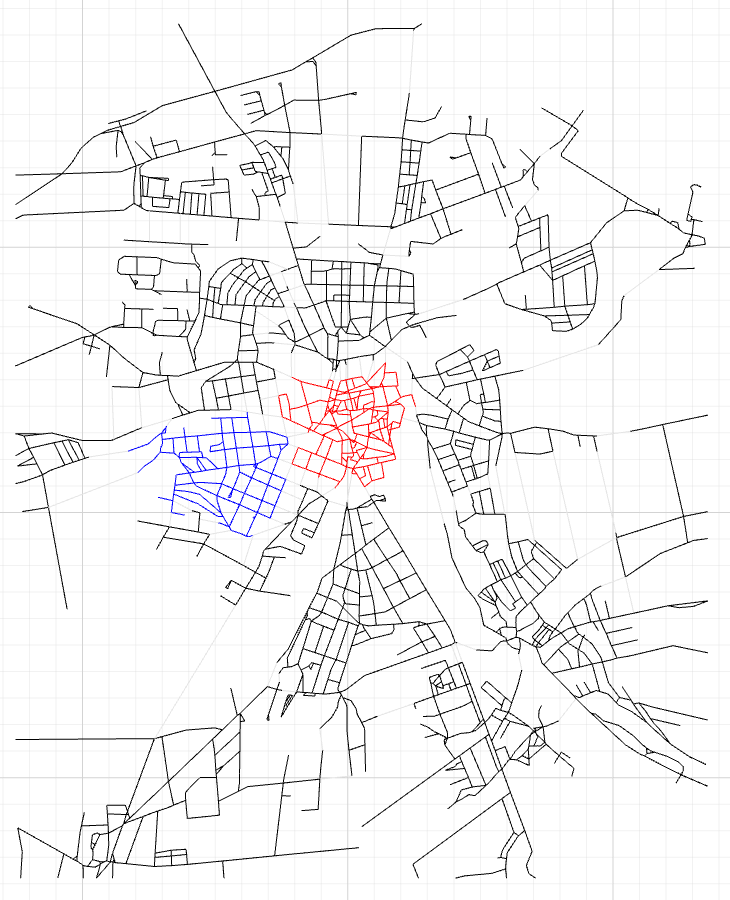
\includegraphics[width=\linewidth]{cluster_applied_compare_visualized.png}
    \end{mdframed}
    \caption{Main view with marked from the 'Cluster Analysis' dialog}
    \label{fig:applied_clustering_analysis_visualized_GUI}
\end{figure}

\FloatBarrier
\section{Measured Clusters} \label{sec:measurements_full_table}
This table represent the full measured data with the cluster analysis method UPGMA (section \ref{sec:hierarchicalClustering}) on Weimar with \textit{Modified Output} and \textit{Number of Clusters} count 16. Addition informations can be found in section \ref{sec:measurements-cluster-analysis}.

\begin{table}[h]
    \begin{center}
        \begin{tabular}{ |l|l|l|l|l| }
            \hline
            \textbf{Parmate}r &
            & \textbf{C1} \ref{sec:historyDistinct}
            & \textbf{C2} \ref{sec:businessDistinct}
            & \textbf{C3} \ref{sec:outskits}  \\ 
            \hline
            \multirow{4}{*}{Total} 
            & Area & 1838.05 & 1956.59 & 7802.74 \\
            & Length & 806.92 & 643.50 & 1069.81 \\
            & Density & 2.28 & 3.04 & 7.29 \\
            \hline
            \multirow{5}{*}{Street Length}
            & Min & 0.66 & 0.69 & 0.73 \\
            & Max & 9.13 & 10.68 & 38.00 \\
            & Mean & 2.72 & 3.85 & 4.82 \\
            & Median & 2.30 & 3.65 & 3.28 \\
            & Sigma & 1.70 & 2.19 & 5.00 \\
            \hline
            \multirow{1}{*}{Vertex} 
            & Connections & 3.04 & 2.84 & 2.45 \\
            \hline
            \multirow{5}{*}{Street Angle} 
            & Min & 0.00 & 0.00 & 0.00 \\
            & Max & 151.80 & 358.84 & 359.80 \\
            & Mean & 119.03 & 123.75 & 137.18 \\
            & Sigma & 124.68 & 131.65 & 129.47 \\
            \hline
            \multirow{5}{*}{Block} 
            & Count & 55 & 35 & 26 \\
            & Area Min & 0.01 & 0.09 & 0.00 \\
            & Area Max & 31.75 & 42.29 & 567.26 \\
            & Area Mean & 6.54 & 13.65 & 76.30 \\
            & A/Ac Min & 0.01 & 0.01 & 0.00 \\
            & A/Ac Max & 0.54 & 0.55 & 0.66 \\
            & A/Ac Mean & 0.18 & 0.23 & 0.18 \\
            \hline
            \multirow{5}{*}{Integration} 
            & Min & 0.46 & 0.48 & 0.60 \\
            & Max & 0.57 & 0.75 & 1.0 \\
            & Mean & 0.49 & 0.59 & 0.78 \\
            \hline
            \multirow{5}{*}{Choice}
            & Min & 0.00 & 0.00 & 0.00 \\
            & Max & 1.00 & 0.67 & 0.34 \\
            & Mean & 0.10 & 0.05 & 0.04 \\
            \hline
        \end{tabular}
        \caption{Measured results from Historic District (C1) \ref{sec:historyDistinct}, Business District (C2) \ref{sec:businessDistinct} and Outskirts Area (C3) \ref{sec:outskits}}
    \end{center}
\end{table}

\pagebreak
\section{Application Improvements}
This chapter was created to inform the reader about certain improvements and observations made in \gls{acr:CPlan} (section \ref{CPlan}).
\begin{itemize}
    \item Some calls to the methods IEnumerable.ToArray() and IEnumerable.ToList() were removed. This method creates a new array / list and stores every item of the IEnumerable in this new collection. As a result the application had an extremely large footprint. To further reduce this overhead some methods were changed to take IEnumerable parameters instead of arrays.
    \item Certain graph and geometry extension methods were fixed. It would be good practice to create unit tests for such methods.
    \item The vector represented by the class Matrix2d is clockwise despite the norm being counter clockwise.
    \item Line intersections of the class Geometry2D was not correct detected an therefore corrected.
\end{itemize}

\chapter{Declaration of academic integrity}
With this statement we declare, that we have independently completed the above article entitled \textit{Analysing Street Networks with Clustering Algorithms}.
The thoughts taken directly or indirectly from external sources are properly marked as such. This article was not previously submitted to another academic institution and has also not yet been published.\\

\begin{center}
    Windisch, August 19, 2016
    
    \vspace{2cm}
    \begin{tabular}{c c}
        \makebox[5.5cm]{\hrulefill} &
        \makebox[5.5cm]{\hrulefill}\\
        Janis Peyer & Samuel Merki
    \end{tabular}
\end{center}
